\documentclass[conference]{IEEEtran}
\IEEEoverridecommandlockouts
% The preceding line is only needed to identify funding in the first footnote. If that is unneeded, please comment it out.
\usepackage{cite}
\usepackage{amsmath,amssymb,amsfonts}
\usepackage{algorithmic}
\usepackage{graphicx}
\usepackage{textcomp}
\usepackage{xcolor}
\usepackage[ngerman]{babel}
\usepackage[utf8]{inputenc}
\usepackage{listings} % Code
\def\BibTeX{{\rm B\kern-.05em{\sc i\kern-.025em b}\kern-.08em
    T\kern-.1667em\lower.7ex\hbox{E}\kern-.125emX}}
 
    
\begin{document}


\title{Implementierung Objektorientierter-Konstrukte in der Java Virtual Machine\\}

\author{\IEEEauthorblockN{Braun Georg}
\IEEEauthorblockA{\textit{Fachhochschule Aachen} \\
Aachen, Deutschland \\
Georg.Braun@alumni.fh-aachen.de}
}

\maketitle

\begin{abstract}
Diese Seminararbeit beschreibt anhand verschiedener Beispiele wie in der Java Virtual Machine Objektorientierte-Konstrukte umgesetzt werden. Neben einer Erläuterung der Klassen-Datei Struktur, werden auch objektorientierte Aspekte des Stacks und Heaps der Java Virtual Machine hervorgehoben. Im Bereich der Methodenaufrufe wird gezeigt wie diese grundsätzlich umgesetzt werden, welche Aufrufvarianten es gibt und wie Überlade-, Überschreibungs- und Konstruktor-Mechanismen funktionieren. Neben dem Methoden-Aspekt wird auch der Umgang (lesend/schreibend) mit Feldern erläutert.
\end{abstract}

\section{Einleitung}
Die Java Virtual Machine ist eine Laufzeitumgebung welche es ermöglicht Bytecode auszuführen. Aus verschiedenen Programmiersprachen (Beispiel Java, Kotlin, ...) kann  Bytecode erzeugt werden. Die Ausführung des Codes wird durch die Portabilität der Java Virtual Machine unabhängig von der zugrunde liegenden Rechnerarchitektur (vorausgesetzt die Java Virtual Machine kann auf dieser betrieben werden). Im Fokus dieses Dokuments steht der Umgang der Java Virtual Machine mit objektorientierten Konstrukten. Dazu wird auf die Struktur der Java Klassen-Dateien, die Java Virtual Machine Grundlagen, Feldzugriffe, Methodenaufrufe und Typüberprüfungen eingegangen.

\section{Aufbau der class Datei}
\label{chKlassenDatei}
Der Programmcode der Hochsprachen wird beim Kompilieren in Bytecode umgewandelt und für jede verwendete Klasse wird eine entsprechende Klassen-Datei (.class) angelegt. Diese Dateien haben eine klar definierte Struktur die in Tabelle \ref{tab1} aufgelistet ist und auf die im Folgenden eingegangen wird.


\begin{table}[htbp]
\caption{Reihenfolge und Länge der class-Datei Inhalte}
\begin{center}
\begin{tabular}{|c|c|}
\hline
\textbf{Element} & \textbf{Länge} \\
\hline
Magic & 4 Bytes\\
\hline
Major, Minor Version & 4 Bytes\\
\hline
Constant Pool & variabel \\
\hline
Access Flags & 2 Bytes \\
\hline
This Klasse & 2 Bytes \\
\hline
Basisklasse (super) & 2 Bytes \\
\hline
Interfaces & variabel \\
\hline
Felder & variabel \\
\hline
Methoden & variabel \\
\hline
Attribute & variabel \\
\hline
\end{tabular}
\label{tab1}
\end{center}
\end{table}

Es gibt zwei Varianten wie Informationen in der Klassen-Datei dargestellt werden. Für manche Informationen ist eine feste Byte-Länge vorgegeben. Andere Informationen wiederum sind in ihrer Größe variabel, sodass die Byte-Länge im Vorfeld nicht bekannt ist. Um trotzdem die Informationen auswerten zu können, stehen vor den jeweiligen Informationen noch Angaben bezüglich der Byte-Länge. Somit ist es möglich auch Informationen variabler Länge abzubilden.
Die Datei startet zunächst mit einem Magic welches die Datei als eine Java-Klassen-Datei identifiziert. Dieses Magic hat den fixen Wert 0xCAFEBABE. Darauf folgen die Major- und Minor-Versionsinformationen welche die verwendete Compilerversion identifiziert. Die nächsten Bytes beschreiben den sogenannten Constant-Pool. Dieser enthält Konstanten die mit der Klasse, beziehungsweise dem Interface assoziiert werden. Der Constant-Pool ist als Array variabler Länge umgesetzt. Auf die Elemente kann später über einen Index-Mechanismus zugegriffen werden. Dabei enthält ein Element zunächst ein Byte welches den Typ spezifiziert. Auf Grundlage dieses Typs werden die darauf folgenden Bytes des Elements interpretiert. Nach dem Constant-Pool werden in der Klassen-Datei die Access-Flags angegeben. Dabei handelt es sich um Flags die beschreiben ob es sich um eine Klasse oder um ein Interface (\verb|ACC_INTERFACE| Flag) handelt. Zudem werden darüber die Zugriffsrechte bekannt gegeben. Beispielsweise wird für einen public Zugriff das Flag \verb|ACC_PUBLIC| verwendet. In den nächsten Bytes steht die this-Information, welche die in dieser Klassen-Datei behandelte Klasse oder Interface definiert. Dazu werden diese Bytes als Index im Constant-Pool interpretiert. Dieser muss an dem gegeben Index ein Element des Typs \verb|CONSTANT_Class| enthalten. Dieser wiederum verweist auf ein String-Element welches den Namen der Klasse beziehungsweise des Interfaces enthält. Die nächsten Bytes geben die verwendete Elternklasse an. Auch hier werden die Bytes als Index im Constant-Pool interpretiert. In diesem Element sollte der Typ \verb|CONSTANT_Class| stehen und auf die Elternklasse verweisen. Nach dieser Angabe folgen die verwendeten Interfaces. In nächsten Bytes erfolgt eine Beschreibung aller Felder die in der Klasse oder dem Interface deklariert wurden. Geerbte Felder werden hier nicht repräsentiert. Ähnlich verhält es sich bei den folgenden Methoden-Definitionen. Diese enthalten (sofern nicht als abstrakt gekennzeichnet) neben der Deklaration auch die komplette Implementation. Dabei werden neben Instanz-Methoden auch Klassen- und Initialisierungsmethoden angegeben. Als letztes kann die Klassen-Datei noch verschiedene Attribute wie zum Beispiel die verwendete Quell-Datei enthalten. \cite{Venners.1996b} \cite{Lindholm.21.08.2018}

\section{Java Virtual Machine Grundlagen Stack und Heap}

% Quelle: JVM SE Specification!
Die Java Virtual Machine besteht aus verschiedenen Bereichen, wobei im Folgenden besonders der Java Virtual Machine Stack und Heap beschrieben wird.

\subsection{Stack}
Bei der Ausführung von Programmen in einer höheren Programmiersprache existieren meist mehrere Threads parallel. Dabei stellt ein Thread einen sequentiellen Ablauf von Instruktionen dar. Auf der Ebene der Java Virtual Machine besitzt jeder Thread einen eigenen Java Virtual Machine Stack der zeitgleich mit der Threaderstellung entsteht. Mit diesen Stacks ist es möglich die parallelen Abläufe voneinander abzugrenzen. Ein solcher Stack enthält \verb|Frames|. Bei jedem Methodenaufruf wird ein neues Frame erstellt und auf dem Stack abgelegt. Ein Frame besteht aus einem Operanden-Stack, einem Array von lokalen Variablen und einer Referenz zum Runtime Constant-Pool. Der Runtime Constant-Pool ist ein Teil des Heap, dessen Beschreibung in Kapitel \ref{chHeap} erfolgt. Der Operanden-Stack ist ein LIFO-Stack der verschiedene Werte aufnehmen kann (Integer, Referenzen, Double, ...). Mit den Befehlen des Bytecodes, den sogenannten Opcodes, kann der Stack manipuliert werden. Die Java Virtual Machine definiert eine Reihe von Opcodes (Rechenoperationen, Methodenaufrufe, ...) mit denen es möglich ist Programmabläufe darzustellen. Das Array der lokalen Variablen hat zwei Funktionen. Zunächst enthält es bei einem Methodenaufruf die übergebenen Parameter. Handelt es sich bei einem Methodenaufruf um eine Instanz-Methode, so ist der erste Wert in dem Array (Index 0) eine Referenz auf das beim Aufruf verwendete Objekt (this-Referenz). Die zweite Funktion ist das Speichern der Werte von lokalen Variablen. 

\subsection{Heap}
\label{chHeap}
In der Java Virtual Machine gibt es einen Heap den sich alle Threads teilen. Bei der Erstellung einer neuen Klassen-Instanz oder eines Arrays wird in diesem Bereich Speicher allokiert. Die Spezifikation der Java Virtual Machine macht keine Vorschriften oder Annahmen über die Repräsentation von Objekten im Heap, da dies ein wesentlicher Aspekt des Gesamstdesigns einer Java Virtual Machine Implementation ist. Somit bleibt die konkrete Umsetzung dem Hersteller überlassen \cite{Lindholm.21.08.2018}. Vorgeschrieben ist jedoch, dass das Objekt über eine Referenz auffindbar sein muss. Außerdem muss das Objekt Instanz-Variablen sichern und eine Referenz auf die zugrundeliegende Klasse beinhalten. In den meisten Implementationen wird für letzteres meist ein Verweis auf die \textit{Method Area} genutzt, welche einen weiterer Bestandteil des Heaps ist und Informationen zu Klassen und Interfaces enthält. Der Verweis auf die Klasseninformation wird beispielsweise notwendig, wenn die potenziell aufrufbaren Methoden ermittelt werden müssen. Zwei potenzielle Umsetzungen werden im Folgenden beschrieben. Eine Möglichkeit ist, dass Referenzen zunächst auf einen sog. Handle-Pool verweisen. Ein Eintrag dort beinhaltet zwei Zeiger: Einen auf das Objekt mit den Instanz-Daten und einen weiteren der auf die zugrundeliegende Klasse verweist. Ein anderer Ansatz ist, dass den Instanz-Daten eine Referenz auf die Klassen-Daten vorangestellt ist.

Neben dem Speicher für Strukturen wie Instanzen und Arrays gibt es im Heap noch die bereits erwähnte \textit{Method Area}, welche im folgenden noch detaillierter beschrieben wird. In der Java Virtual Machine Spezifikation werden dort Informationen von Klassen, Interfaces, Runtime Constant-Pool, Feld- und Methodendaten, Methodencode, Konstruktorcode und Methoden-Tabellen verwaltet. Beim Runtime Constant Pool handelt es sich um eine Laufzeit-Repräsentation des in den Klassendateien definierten Constant Pools (siehe Kapitel \ref{chKlassenDatei}). Dieser Runtime Pool wird angelegt sobald eine Klasse oder ein Interface erstellt wird. Wird eine nicht abstrakte Klasse durch die Java Virtual Machine geladen, so wird zeitgleich eine Methoden-Tabelle erstellt und mit der geladenen Klasse verknüpft. Bei dieser Tabelle handelt es sich um ein Array von Referenzen zu allen Instanz-Methoden die potenziell auf einer Instanz aufgerufen werden können. Das schließt auch Methoden ein die von anderen Klassen geerbt wurden. Dabei ist laut der Spezifikation jedoch die grundsätzliche Umsetzung, beziehungsweise die Art der Implementation nicht vorgegeben. Eine potenzielle Umsetzung ist in Abbildung \ref{fig:linkZurMethodenTabelle} zu sehen. Durch die Objekt-Referenz kann auf die Daten im Heap zugegriffen werden. Dort wird eine hinterlegte Klassen-Referenz genutzt um die Klasse in der \textit{Method Area} zu identifizieren. Dort kann auf die Methoden-Tabelle zugegriffen werden, über die letztendlich auf die jeweiligen Methoden verwiesen wird.
\begin{figure}[htbp] 
  \centering
     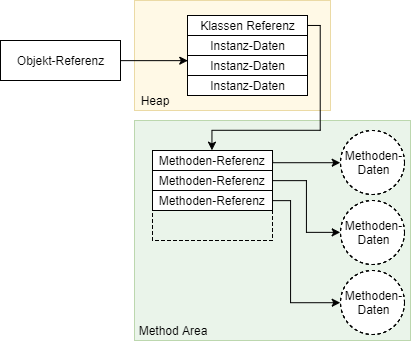
\includegraphics[width=0.45\textwidth]{Grafiken/LinkZurMethodenTabelle.png}
  \caption{Referenz zur Methoden-Tabelle}
  \label{fig:linkZurMethodenTabelle}
\end{figure}

Die Java Virtual Machine Spezifikation definiert nur Instruktionen um Speicher zu allokieren, aber nicht um diesen auch wieder freizugeben. Eine Implementation der Java Virtual Machine muss selber prüfen ob Objekte die nicht mehr referenziert werden freigegeben werden können. Die Implementation des Garbage Collectors ist jedoch nicht vorgeschrieben, sodass sich die Umsetzung je nach genutzter Java Virtual Machine unterscheiden kann. \cite{Venners.1999} 

\section{Methodenaufrufe}
\subsection{Ablauf eines Methodenaufrufs}
Für den Aufruf von Methoden werden im Bytecode verschiedene \textit{invoke} Funktionen genutzt die sich in ihrem Verhalten unterscheiden. Gemeinsam haben diese Opcodes jedoch, dass sie als Operanden einen Index  im Runtime Constant Pool haben. Dieser Index wiederum verweist auf eine Methoden-Referenz, über die dann der konkrete Methodencode ermittelt werden kann. Sobald eine Methode aufgerufen wird erzeugt die Java Virtual Machine ein neues Frame und legt dieses auf den Frame-Stack. Sofern es sich um eine Instanz-Methode handelt, werden im Kontext der aufrufenden Methode und in dessen Frame die Objekt-Referenz und potenzielle Methodenargumente von dem Operanden-Stack genommen und in den Frame der aufgerufenen Methode übergeben (siehe Abbildung \ref{fig:aufrufMethode}). Dort sind die Werte im Array der lokalen Variablen zu finden, wobei die Objekt-Referenz an erster Stelle (Index 0) steht und darauf folgend die potenziellen Methoden-Argumente. 

\begin{figure}[htbp] 
  \centering
     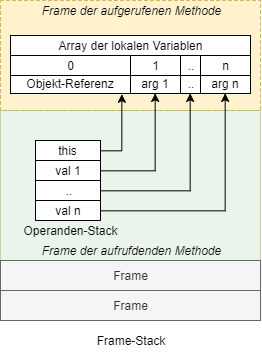
\includegraphics[width=0.3\textwidth]{Grafiken/MethodenAufrufJVM.png}
  \caption{Aufruf einer Instanz-Methode}
  \label{fig:aufrufMethode}
\end{figure}

Falls es sich um den Aufruf einer Klassen-Methode handelt, werden nur die Argumente vom Operanden-Stack genommen und das Array der lokalen Variablen in dem Frame der aufgerufenen Methode startet ab Index 0 mit den Methoden-Argumenten. Sobald die Argumente in dem Array vorhanden sind, aktiviert die Java Virtual Machine das neu erzeugte Frame und setzt den Instruktionszeiger auf die erste Instruktion der neuen Methode.\cite{Venners.1997}

\subsubsection{Dynamic linking}
Die Java Virtual Machine nutzt dynamisches Linken. Wie bereits zuvor erwähnt haben die \textit{invoke} Opcodes eine Referenz im Runtime Constant Pool als Operanden. Die dort enthaltenen Verweise auf die Methode sind zu Beginn jedoch nur symbolisch (symbolische Referenzen). Eine solche symbolische Referenz ist eine Sammlung von Informationen, welche unter anderem den Klassennamen, Methodennamen und Methoden-Deskriptor enthält. Der Methoden-Deskriptor enthält den Rückgabewert der Methode, sowie Anzahl und Typen der Methoden-Argumente). Wird nun eine Methode zur Laufzeit das erste Mal aufgerufen, muss die symbolische Referenz erst aufgelöst werden. Durch die Informationen in der Referenz kann die Java Virtual Machine nach der benötigten Methode suchen und anschließend die symbolische Referenz durch eine direkte Referenz ersetzen. Somit ist für einen weiteren Aufruf der Methode keine erneute Suche notwendig.\cite{Venners.1997}


\subsection{Vergleich der Methodenaufrufe}
In der Java Virtual Machine kann man zunächst die zuvor angesprochenen zwei Arten von Methoden unterscheiden: Instanz-Methoden und Klassen-Methoden. Sie unterscheiden sich zunächst darin, ob für ihren Aufruf eine Instanz benötigt wird oder nicht. 

Wie bereits zuvor erwähnt können Instanz-Methoden nur in ihrem Instanz-Kontext aufgerufen werden, wobei die aufgerufene Methode von der aktuellen Klasse der Instanz abhängt. Diese Information ist jedoch erst zur Laufzeit des Programms bekannt. Für die Lösung des Problems wird der Mechanismus des \textit{late bindings} genutzt. Dabei wird beim Aufruf einer Methode der aktuelle Typ des Objekts ermittelt und dieser nach der Methode durchsucht. Die grobe Funktionsweise wird in Abbildung \ref{fig:linkZurMethodenTabelle} erläutert. Dieser Mechanismus ist sehr ähnlich zu den \textit{Tabellen virtueller Methoden} in C++. Anhand des folgenden Beispiels wird die Funktionsweise von \verb|invokevirtual|, der Umgang mit Methodenüberladung und Methodenüberschreibung verdeutlicht. Als Ausgangslage dient das Klassenkonstrukt in Abbildung \ref{fig:umlHierarchie}, wobei die Klasse Student von der Klasse Mensch erbt und diese wiederum von der Basisklasse Object.
\begin{figure}[htbp] 
  \centering
     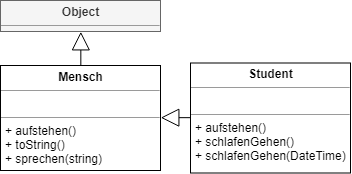
\includegraphics[width=0.45\textwidth]{Grafiken/UMLHierarchie.png}
  \caption{Klassenkonstrukt Beispiel}
  \label{fig:umlHierarchie}
\end{figure}
Eine Methodentabelle für die Klasse Student könnte dann wie in Abbildung \ref{fig:methodenTabelleUmlHierachie} dargestellt aussehen. Dort sind die Methoden-Referenzen aufgelistet  welche für die Klasse Student zur Verfügung stehen. Jede Methode ist dabei einer bestimmten Position (Offset) zugeordnet. Die Reihenfolge der Methoden sind nach ihrem Vorkommen in der Vererbungshierarchie geordnet. Diese beginnt mit Methoden der Klasse Object und endet mit den Methoden der Klasse Student. Die gelb markierten Methoden weisen auf überschriebene Methoden hin. Wird zum Beispiel ein Methoden-Aufruf von \verb|toString| benötigt, so wird auf die Implementation in der Klasse \verb|Mensch| verwiesen und nicht auf die Standardimplementation der Klasse \verb|Object|. Somit wird deutlich wie überschriebene Methoden-Aufrufe realisiert werden. Auch überladene Methoden-Aufrufe sind möglich wie die Methode \verb|schlafenGehen| zeigt. Dieser Methodenname ist doppelt vorhanden, jedoch unterscheiden sich die Methoden in ihrer Signatur, sodass ein differenzierter Aufruf der Methode möglich ist.\cite{Venners.1999}
\begin{figure}[htbp] 
  \centering
     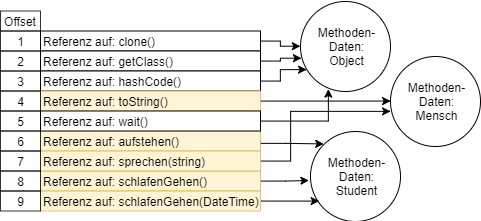
\includegraphics[width=0.45\textwidth]{Grafiken/MethodenTabelleAusHierarchie.png}
  \caption{Methodentabelle der Klasse Student}
  \label{fig:methodenTabelleUmlHierachie}
\end{figure}

Aufrufe von Klassen-Methoden hingegen basieren auf dem verwendeten Typ einer Referenz (Variablen), welcher sich auch während der Laufzeit nicht ändert. Die Instanziierung \verb|Mensch oneHuman = new Student();| erzeugt zwar ein Objekt der Klasse Student, der Typ der Referenz (\verb|oneHuman|) ist aber die Klasse Mensch. Somit kann bereits während der Kompilierung die genutzte Methode bestimmt werden und es ist kein dynamisches Binden notwendig. Hierbei spricht man auch von \textit{static (early) binding}. Der verwendete Opcode zum Aufruf von Klassen-Methoden ist \verb|invokestatic|. \cite{Venners.1997}

\subsubsection{Spezialisierte Aufrufe}
Neben dem zuvor erwähnten Opcode \verb|invokevirtual| zum Aufruf von Instanz-Methoden gibt es noch zwei weitere Varianten dieses Opcodes, welche je nach Kontext verwendet werden. 

Der erste Opcode ist \verb|invokespecial|, welcher in Situationen genutzt wird in denen es notwendig ist eine Instanz-Methode basierend auf dem Typ der Referenz (und nicht des Objekts) aufzurufen (siehe Instanziierungs-Beispiel). In diesem Fall wird auch kein dynamisches Binden benötigt. Eine solche Situation ist zum Beispiel die Instanz-Initialisierung, welche über die sogenannten Init-Methoden erfolgt. Diese Methoden enthalten den Konstruktur-Code. Jede Klasse hat für jeden Konstruktur eine eigene Implementation dieser Methode (wird kein Konstruktor explizit definiert, wird eine Standardimplementation angelegt). Sobald eine neue Instanz erzeugt wird, findet der Aufruf dieser Methode statt. Innerhalb dieser wird entlang der Vererbungshierarchie die Initialisierungs-Methode der vererbenden Klasse aufgerufen. Für diesen Aufruf ist die Verwendung von \verb|invokespecial| vorgesehen. Eine ähnliche Situation für die Verwendung des Opcode ist der Aufruf von überschriebenen Instanz-Methoden. Wird die Implementation der vererbenden Klasse mit dem Schlüsselwort \textit{super} aufgerufen, so findet der Aufruf im Bytecode ebenfalls mit \verb|invokespecial| statt.

% ToDo: invokeinterface
Eine weitere Variante ist die Verwendung von \verb|invokeinterface|. Diese wird verwendet wenn die zugrundeliegende Referenz ein Interface ist. Ansonsten ist die Funktionsweise sehr ähnlich zu \verb|invokevirtual|. Wenn die Java Virtual Machine eine Klassen-Datei lädt, wird (je nach der verwendeter Java Virtual Machine Implementation) eine Methoden-Tabelle für die Klasse erzeugt. Diese Tabelle enthält die direkten Referenzen zu den Bytecodes der Methoden, welche bei einer Instanz dieser Klasse aufgerufen werden können. Die Tabelle beinhaltet dabei auch die Methoden der Oberklassen. Findet ein Methoden-Aufruf auf Basis einer Klassen-Referenz statt, ist die Reihenfolge der Methodendefinitionen fix, sodass die Java Virtual Machine sich sicher sein kann an welcher Stelle (Offset) in der Tabelle die benötigte Methode steht. Die gleiche Methode kann aber gegebenenfalls auch über unterschiedliche Interfaces angesprochen werden, wobei nicht unbedingt eindeutig ist an welcher Position in der Methoden-Tabelle die Methode zu finden ist. Deshalb muss die Methode bei jedem Aufruf über ein Interface neu gesucht werden, was wiederum einen gesonderten Aufruf mit dem Opcode \verb|invokeinterface| notwendig macht.\cite{Venners.1997}

\section{Konstruktor}
In vielen Programmiersprachen werden neue Objekte mit dem Schlüsselwort \verb|new| erzeugt (Beispiel Java). Dieses Schlüsselwort gibt es auch als Opcode auf Bytecode-Ebene. Die \verb|new| Anweisung sorgt dafür dass ein Objekt angelegt wird, aber nicht dafür dass es auch initialisiert wird. Dafür sind die bereits vorgestellten \verb|init| Methoden verantwortlich. Anhand der Erzeugung einer Instanz der Klasse \verb|Student| (siehe Abbildung \ref{fig:umlHierarchie}) werden die einzelnen Schritte im Bytecode aufgezeigt.

Der in Java implementierte Aufruf
\begin{lstlisting}
Student sA = new Student();
\end{lstlisting}
sieht in der Bytecode Implementation wie folgt aus:
\begin{lstlisting}
new           #2                  
dup
invokespecial #3                 
astore_0
\end{lstlisting}
Zudem sind folgende Einträge im Constant-Pool zur Erstellung der Instanz relevant:
\begin{lstlisting}
#2 = Class          #23
#3 = Methodref      #2.#22
#8 = Utf8           <init>
#9 = Utf8           ()V
#22 = NameAndType   #8:#9
#23 = Utf8          com/company/Student
\end{lstlisting}
Der Opcode \verb|new| hat den Index 2 im Constant-Pool als Operanden. Der dazugehörende Eintrag gibt mit dem Typ \verb|Class| an, dass es sich um eine Klasseninformation handelt. Dieser Eintrag wiederum verweist auf Index 23 in dem als Utf8 codierter String der Klassenbezeichner (\verb|com/company/Student|) enthalten ist. Über das bereits vorgestellte dynamische Linken ist es nun möglich die Informationen zu dieser Klasse abzurufen. Der \verb|new| Opcode erzeugt somit die neue Instanz im Heap und legt auf dem Operanden Stack eine Referenz zu dieser ab. Der nächste logische Schritt wäre eigentlich der Aufruf der Initialisierungsmethode \verb|init|. Jedoch erwartet der Aufruf der \verb|init| Methode mit dem \verb|invokespecial| Opcode eine Objekt-Referenz als Parameter auf dem Operanden-Stack. Dies ist in der aktuellen Situation auch der Fall, jedoch wird mit dem Aufruf auch der Parameter vom Operanden-Stack genommen und danach nicht wieder zurückgelegt. Um trotzdem nach dem Aufruf noch die Referenz zu dem erstellten Objekt zu haben, wird die Referenz nach der Erstellung mit \verb|new| zunächst dupliziert (\verb|dup|). Als Resultat ist die gleiche Objekt-Referenz doppelt auf dem Operanden-Stack vorhanden. Somit kann die \verb|init| Methode aufgerufen werden, ohne dass die Referenz zu dem Objekt verloren geht. Der letzte Schritt ist die Sicherung der Objekt-Referenz an Index-Position 0 im Array der lokalen Variablen (\verb|astore_0|).


\section{Zugriff auf Felder}
\subsection{Zugriff auf Objekt-Felder}
Für den Zugriff auf Felder eines Objekts werden die Opcodes \verb|putfield| und \verb|getfield| verwendet. Die Funktionsweise der beiden Opcodes wird wieder an einem konkreten Beispiel gezeigt. Dazu werden die bereits zuvor verwendeten Klassen Mensch und Student um folgendes String-Feld ergänzt:
\begin{lstlisting}
public String Name;
\end{lstlisting}
Somit haben beide Klassen ein Feld mit der Bezeichnung \textit{Name}. Im Folgenden wird auf das neue Feld lesend zugegriffen, um den Inhalt in einer Variablen zu sichern:
\begin{lstlisting}
Student sA = new Student();
var x = sA.Name;
\end{lstlisting}
Der daraus resultierende Bytecode zum Zugriff auf das Feld und Teile des Constant-Pools sehen wie folgt aus:
\begin{lstlisting}
aload_0
getfield      #4
astore_1

#4 = Fieldref       #2.#27         
#2 = Class          #26   
#26 = Utf8          com/company/Student         
#27 = NameAndType   #33:#21        
#21 = Utf8          Ljava/lang/String;
#33 = Utf8          Name
\end{lstlisting}
Zunächst wird die Referenz des Objekts (welche sich im nullten Index des Arrays der lokalen Variablen befindet) auf den Operanden-Stack gelegt damit eindeutig ist welches Objekt genutzt wird. Danach wird der \verb|getfield| Opcode gefolgt von dem Index 4 aufgerufen. Dieser Index enthält Informationen um welches Feld es sich handelt. Die Informationen werden über weitere Einträge aufgelöst bis letztendlich klar ist, dass auf das Feld \verb|Name| der Klasse \verb|Student| zugegriffen wird. Der ermittelte Wert der Instanz wird auf dem Operanden-Stack abgelegt und dann mit \verb|astore_1| in das Array der lokalen Variablen auf Indexposition 1 abgelegt. Die Indexposition entspricht der Variablen \verb|x| im ursprünglichen Java-Programm.

Ein schreibender Zugriff auf das Feld wird mit \verb|putfield| realisiert. Das Java-Programm wird um die Anweisung \verb|sA.Name = "Peter"| ergänzt, sodass folgender Bytecode und Constant-Pool Eintrag entsteht:
\begin{lstlisting}
aload_0
ldc           #5
putfield      #4

#5 = String             #28
#28 = Utf8              Peter
\end{lstlisting}
Wieder wird die Objekt-Referenz auf den Operanden-Stack gelegt. Mit dem Opcode \verb|ldc| und dem folgenden Index wird ein Wert aus dem Constant-Pool entnommen und auf den Operanden-Stack gelegt. In dem konkreten Beispiel wird der String \textit{Peter} auf dem Stack abgelegt. Somit befinden sich auf dem Operanden-Stack die Objekt-Referenz und der String als Parameter. Diese beiden Elemente werden durch den \verb|putfield| Opcode konsumiert. Die Vorgehensweise für den Feldzugriff ist identisch zum \verb|getfield| Beispiel. 

Dieses Beispiel zeigt auch wie mit einer redundanten Feld Definition umgegangen wird. Sowohl die Mensch-, als auch die Student-Klasse wurden um das gleiche Feld ergänzt. Bei der Verwendung des Feld bei einer Studenten-Instanz wird jedoch nur das Feld der Student-Klasse berücksichtigt. Somit wird deutlich, dass das Feld der vererbenden Klasse überdeckt wird. Zudem wird bei einem Feldzugriff nicht nur der Feldname, sondern auch der Klassenname verwendet (siehe Feldauflösung im Beispiel). Das zeigt, dass es sich nicht um ein doppeltes, sondern um zwei eigenständige Felder handelt. \cite{Venners.1996}


\subsection{Zugriff auf Klassen-/Static-Felder}
Die Funktionsweise für den Zugriff auf Klassen-Felder ist dem Zugriff auf Objekt-Felder sehr ähnlich. Der Hauptunterschied ist, dass für einen lesenden Zugriff auf ein Klassen-Feld der Opcode \verb|getstatic|, beziehungsweise für einen schreibenden Zugriff \verb|putstatic| verwendet wird. Beide Opcode haben wieder einen Index als Operanden der auf einen Eintrag im Constant-Pool verweist. Im Gegensatz zu \verb|getfield| und \verb|putfield| wird aber keine Objekt-Referenz auf dem Operanden-Stack erwartet, da die Aufrufe unabhängig von einem Objekt sind. Lediglich die Klasse und das verwendete Feld müssen über die Constant-Pool Einträge identifiziert werden.

\bibliographystyle{ieeetr}
\bibliography{literatur} 

\end{document}
